\documentclass[a4wide]{report}

\usepackage{amsmath}
\usepackage[a4paper, total={7in, 10.2in}]{geometry}
\usepackage{graphicx}
\usepackage[portuguese]{babel}
\usepackage[utf8]{inputenc}


\begin{document}

\noindent
{\bf Rafael V. Cacilhas  - Relatório 15 (\today)}

\vspace{0.5cm}

\section*{Exercício 1}

\subsection*{a) }
Na Figura \ref{1a} está representado o perfil de densidade $\rho_k$ em função de x para diferentes tempos. Como pode ser visto, o pico de densidade parece se deslocar para a esquerda à medida em que o meio se torna cada vez mais homogêneo. 
\begin{figure}[!htb]
\centering
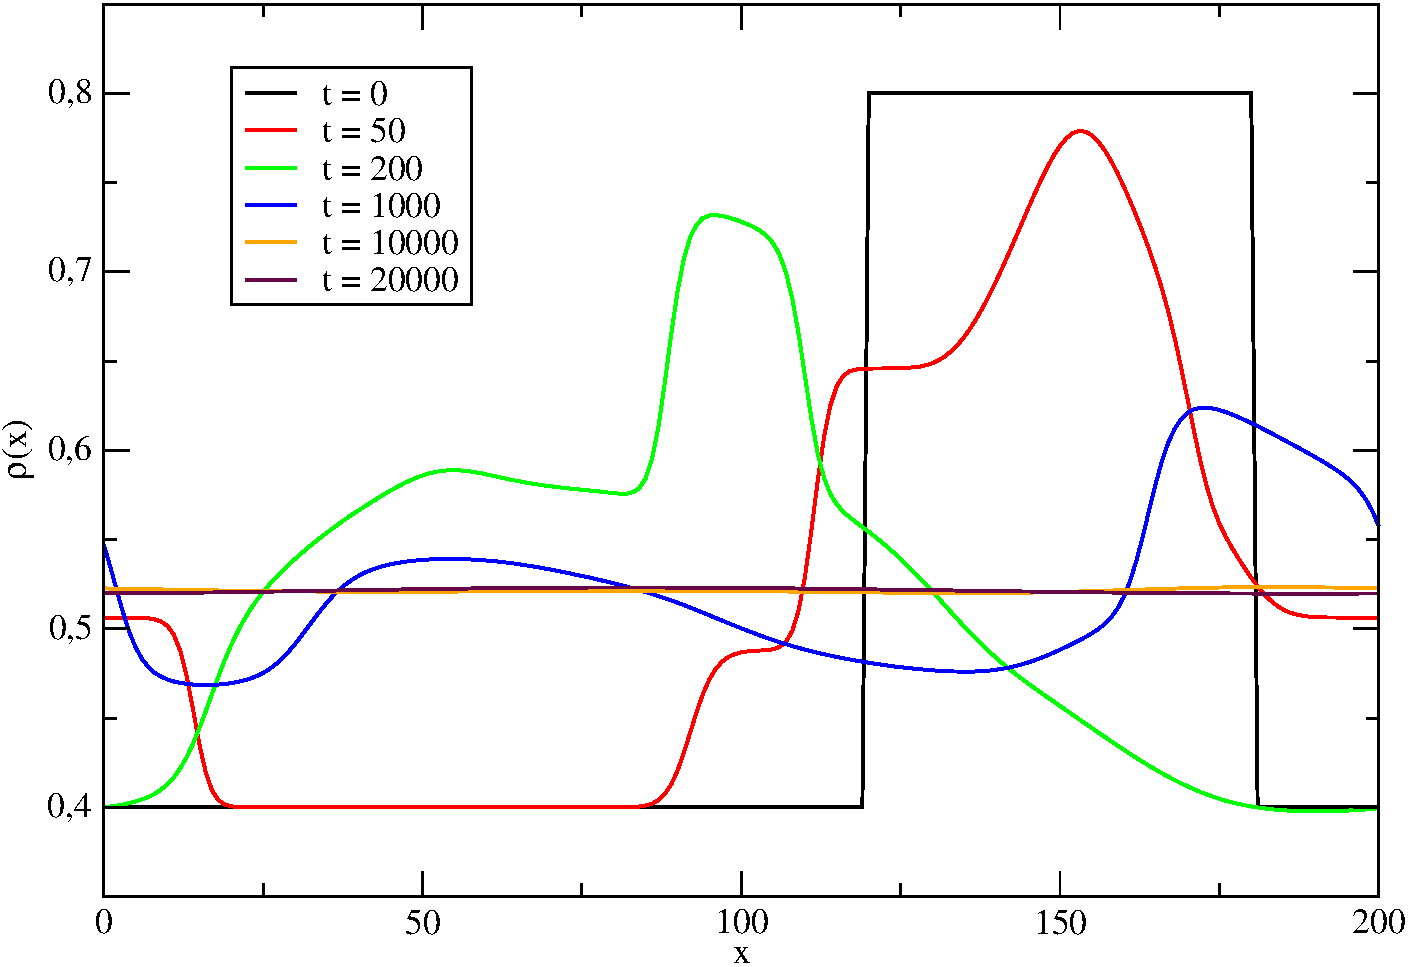
\includegraphics[width=0.6\textwidth]{perfil.pdf}
\caption{Perfil de densidade $\rho_k$ em função de l para diferentes tempos .}
\label{1a}
\end{figure}

A tabela de dados para outros valores de tempo estão na pasta 1/data, caso sejam necessários.

\subsection*{b) }
Na Figura \ref{1b} foram plotados os mapas bidimensionais da densidade $\rho_k$ para cada posição. A escala de cores começa em $\rho_k = 0.4$ (na cor azul) e vai até $\rho_k = 0.8$ (na cor vermelha). Assim como pôde ser visto na Figura \ref{1a} é possível ver aqui mais claramente como a região de maior densidade parece se mover para a esquerda à medida em que o meio se torna mais homogêneo.

\begin{figure}[!htb]
\centering
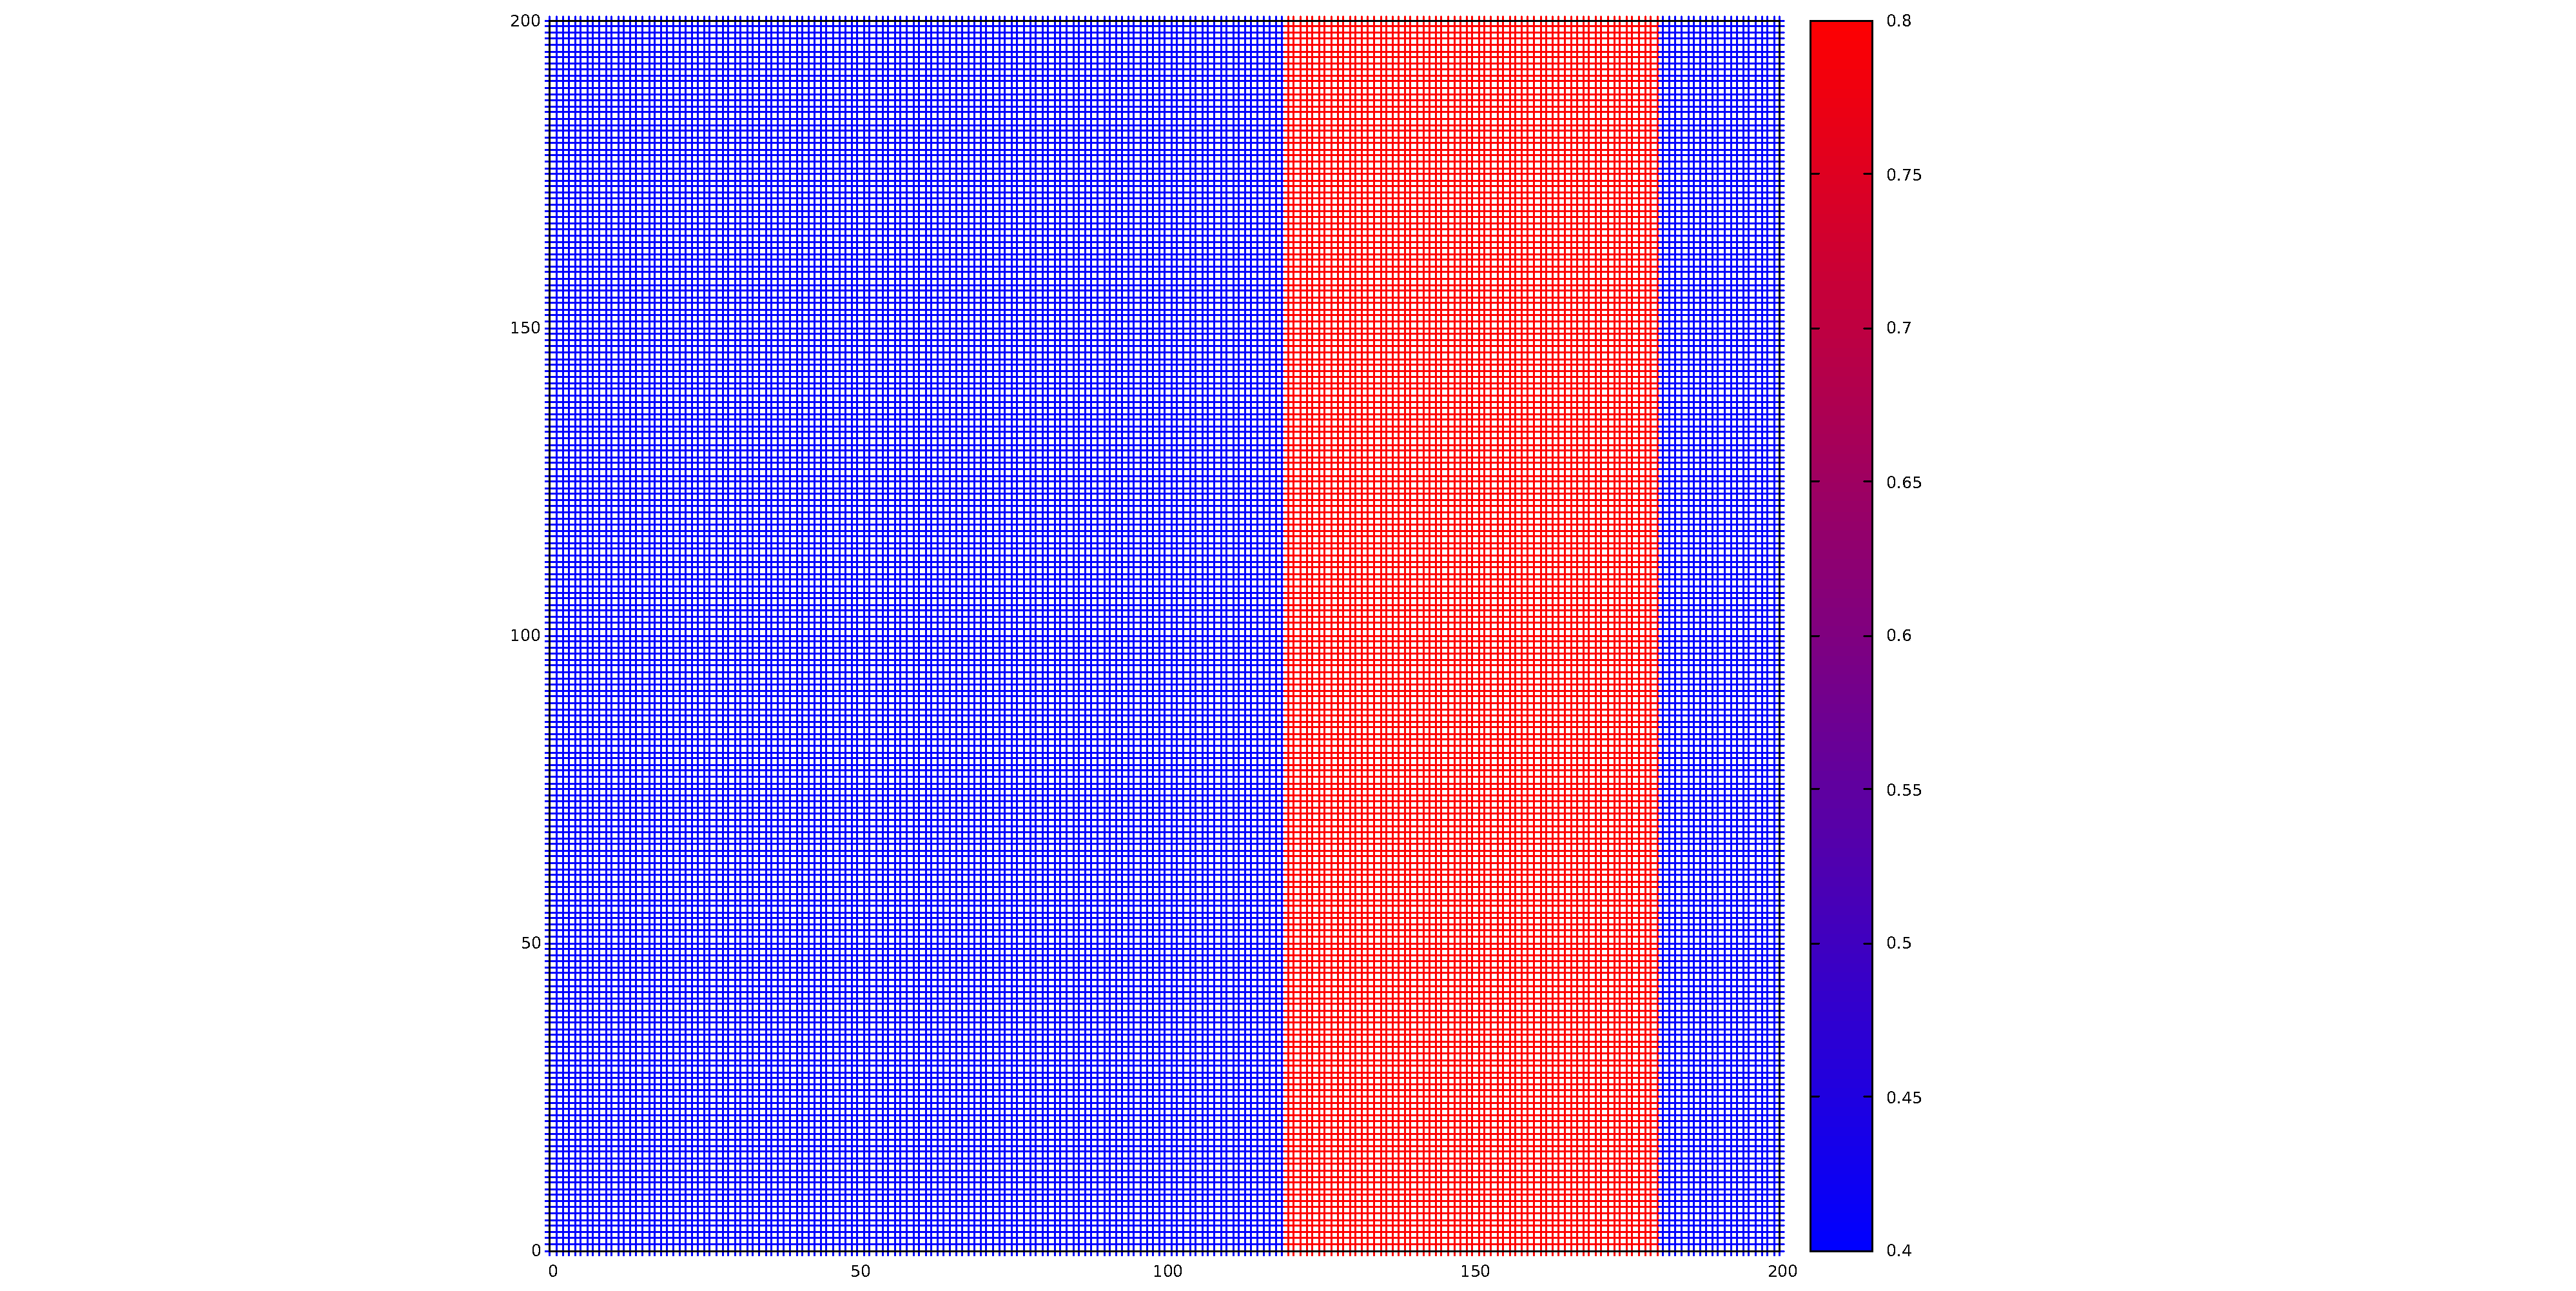
\includegraphics[width=0.4\textwidth]{mapa1.pdf}
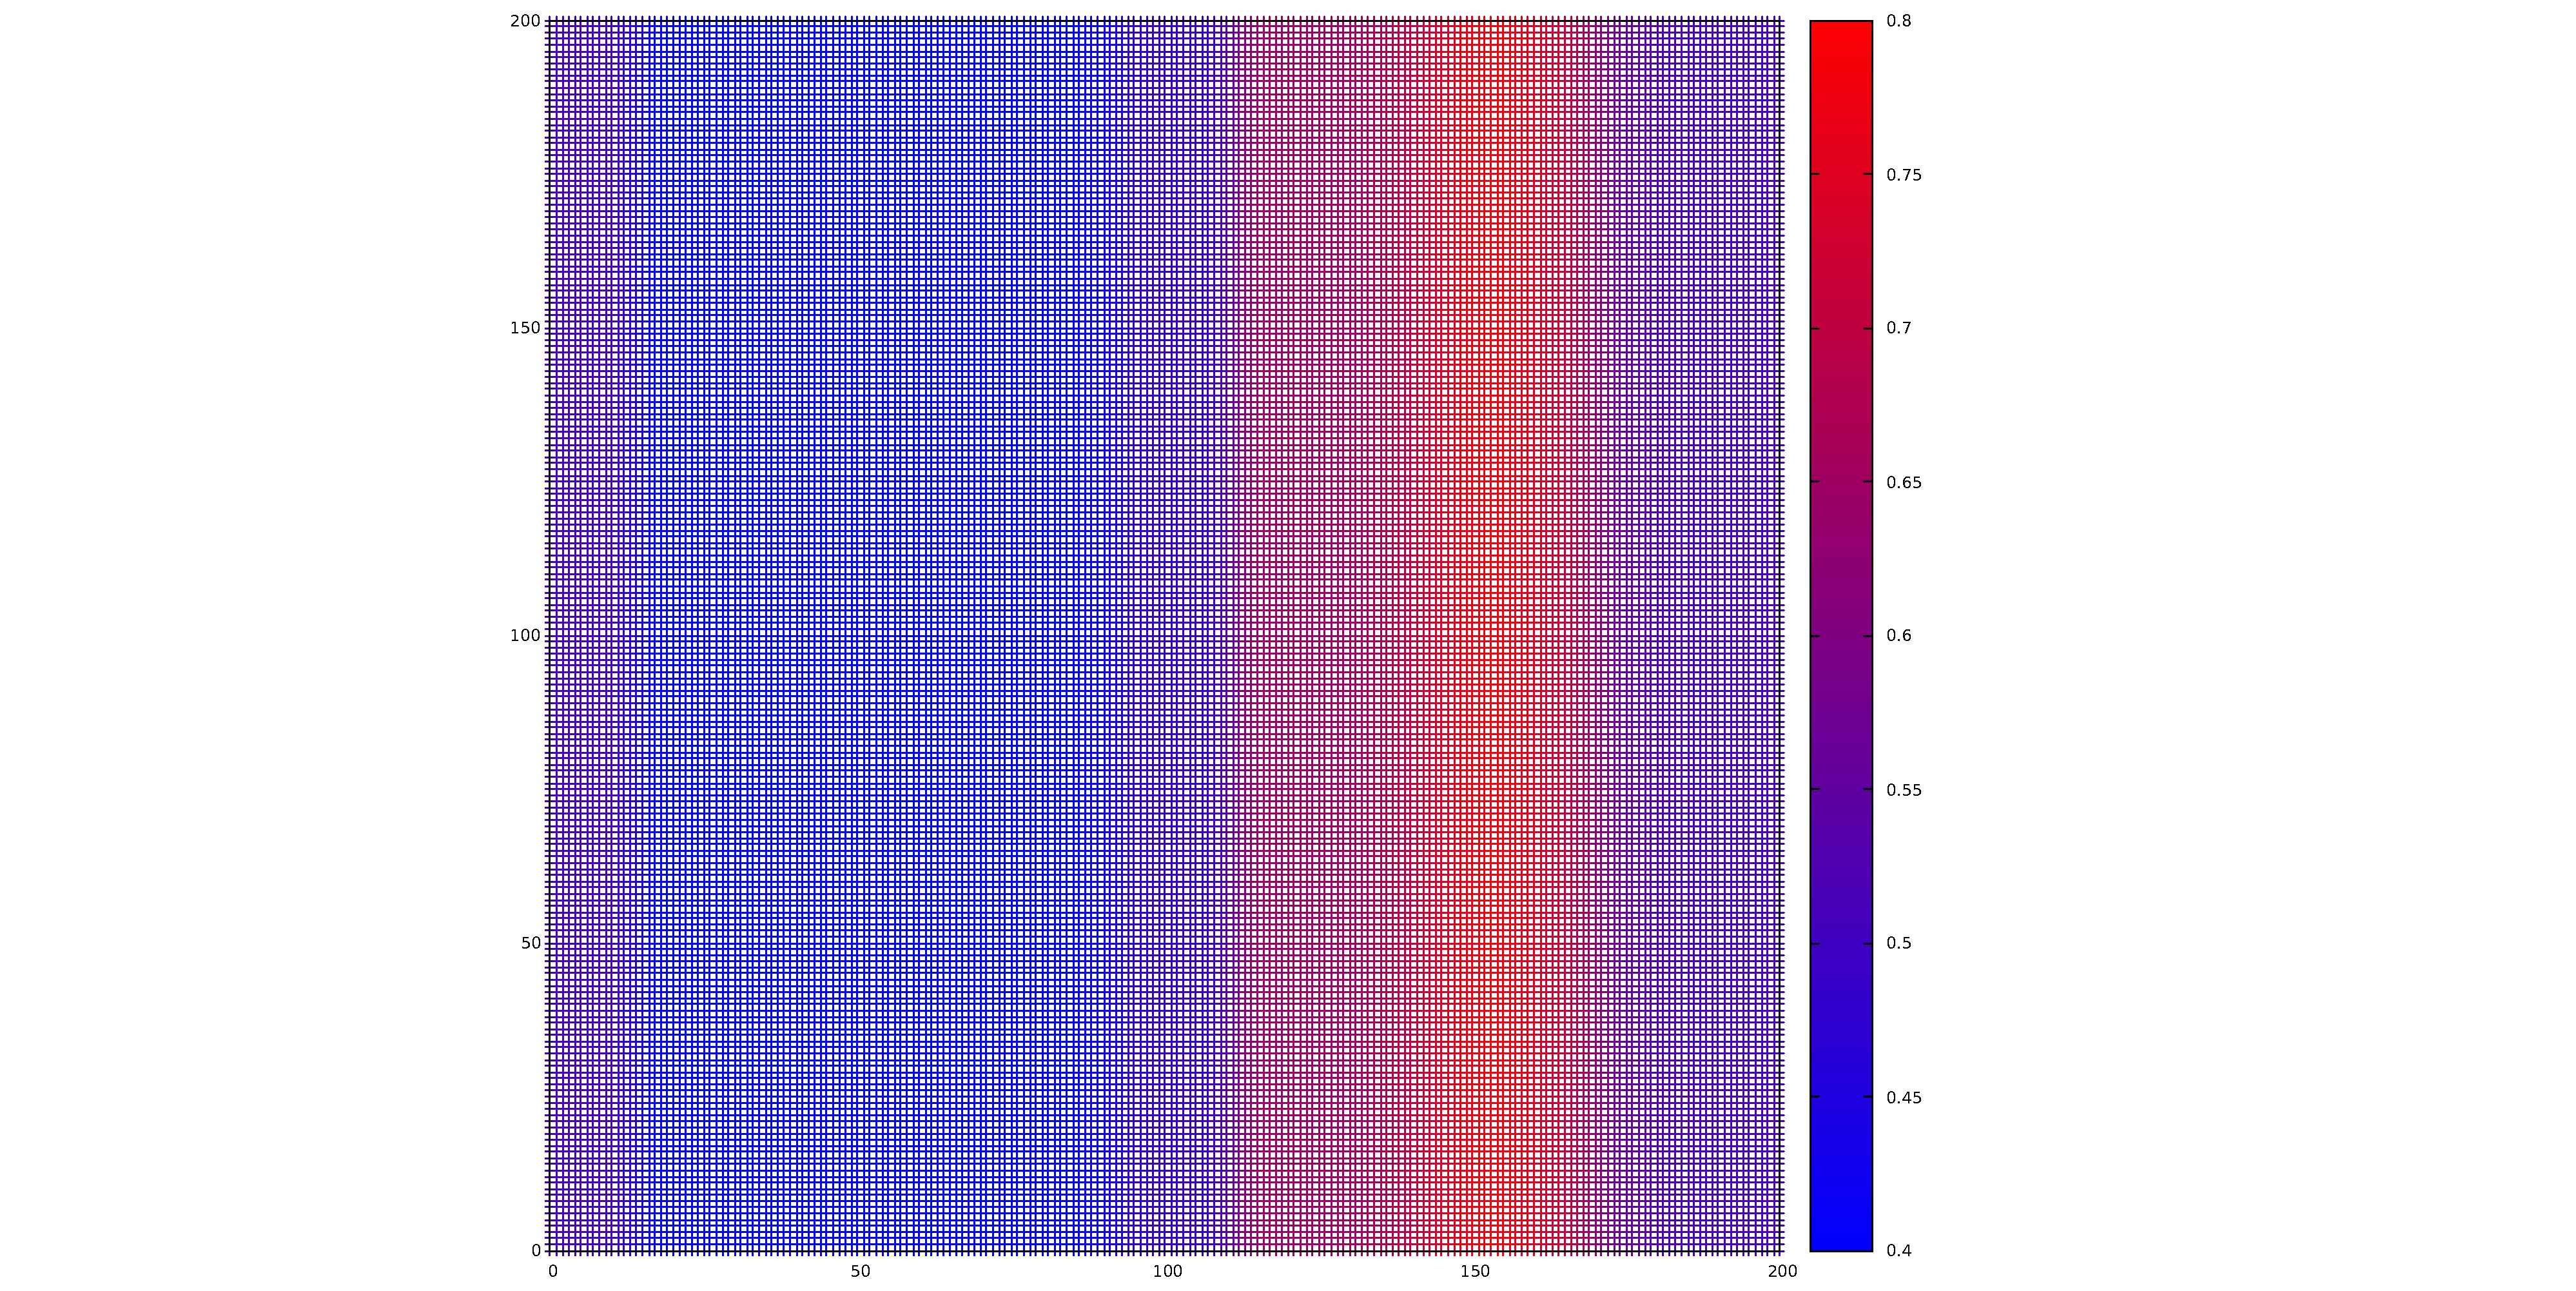
\includegraphics[width=0.4\textwidth]{mapa50.pdf}
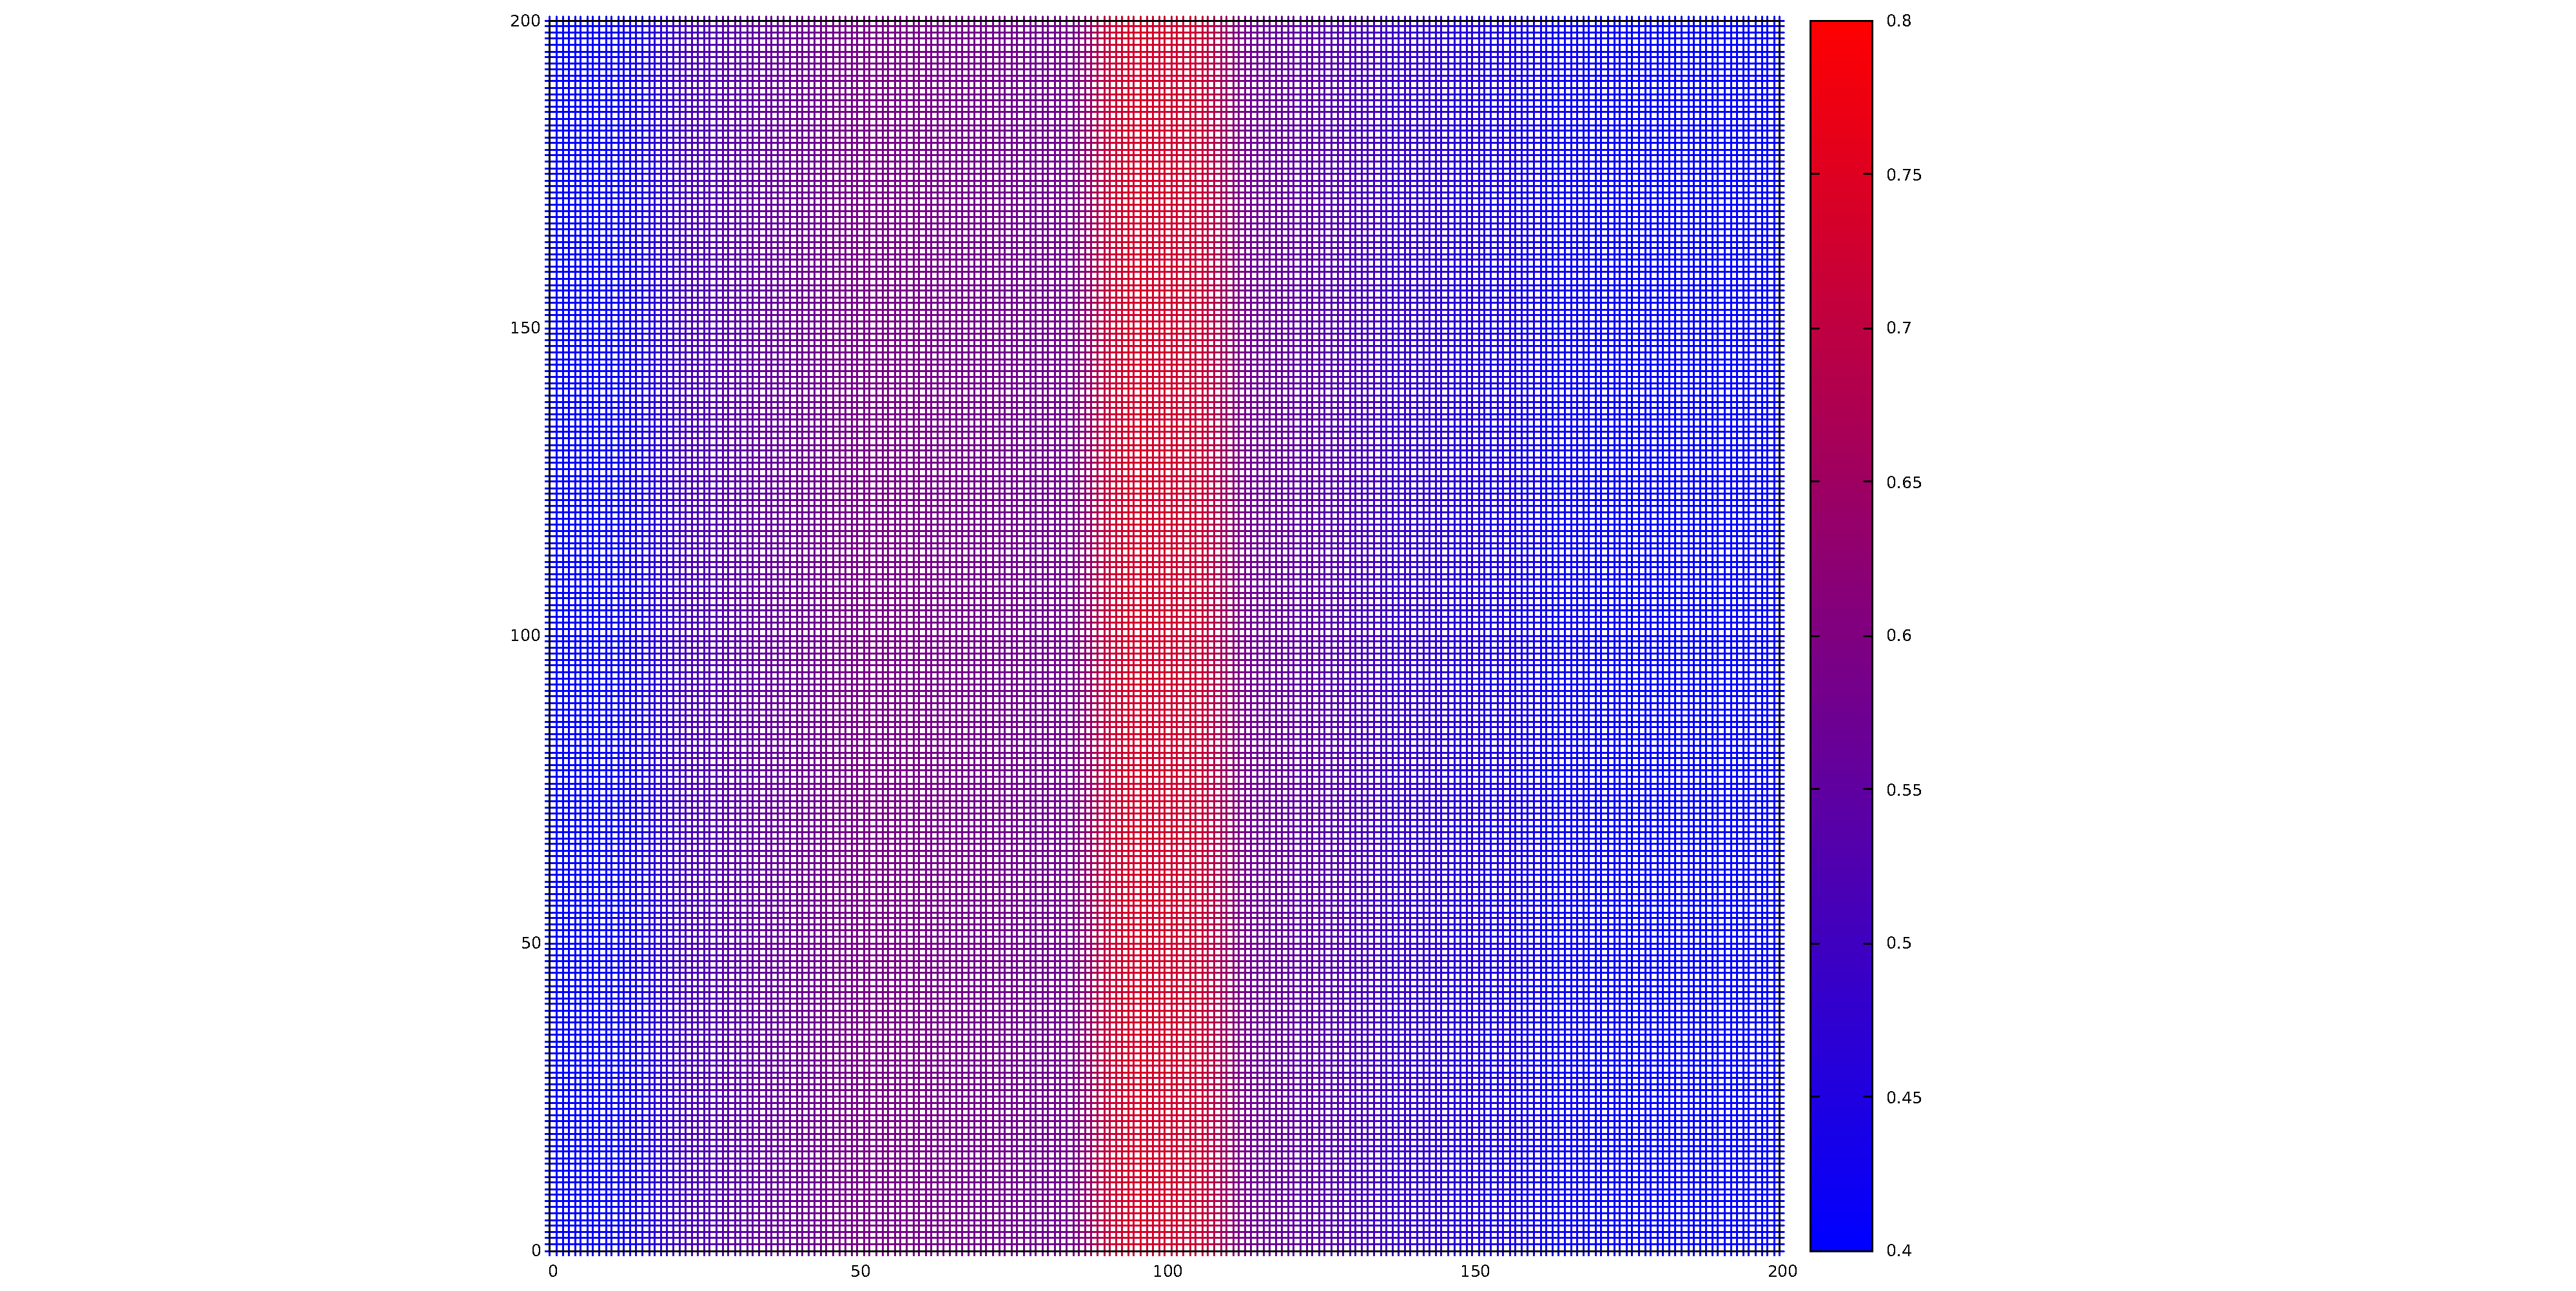
\includegraphics[width=0.4\textwidth]{mapa200.pdf}
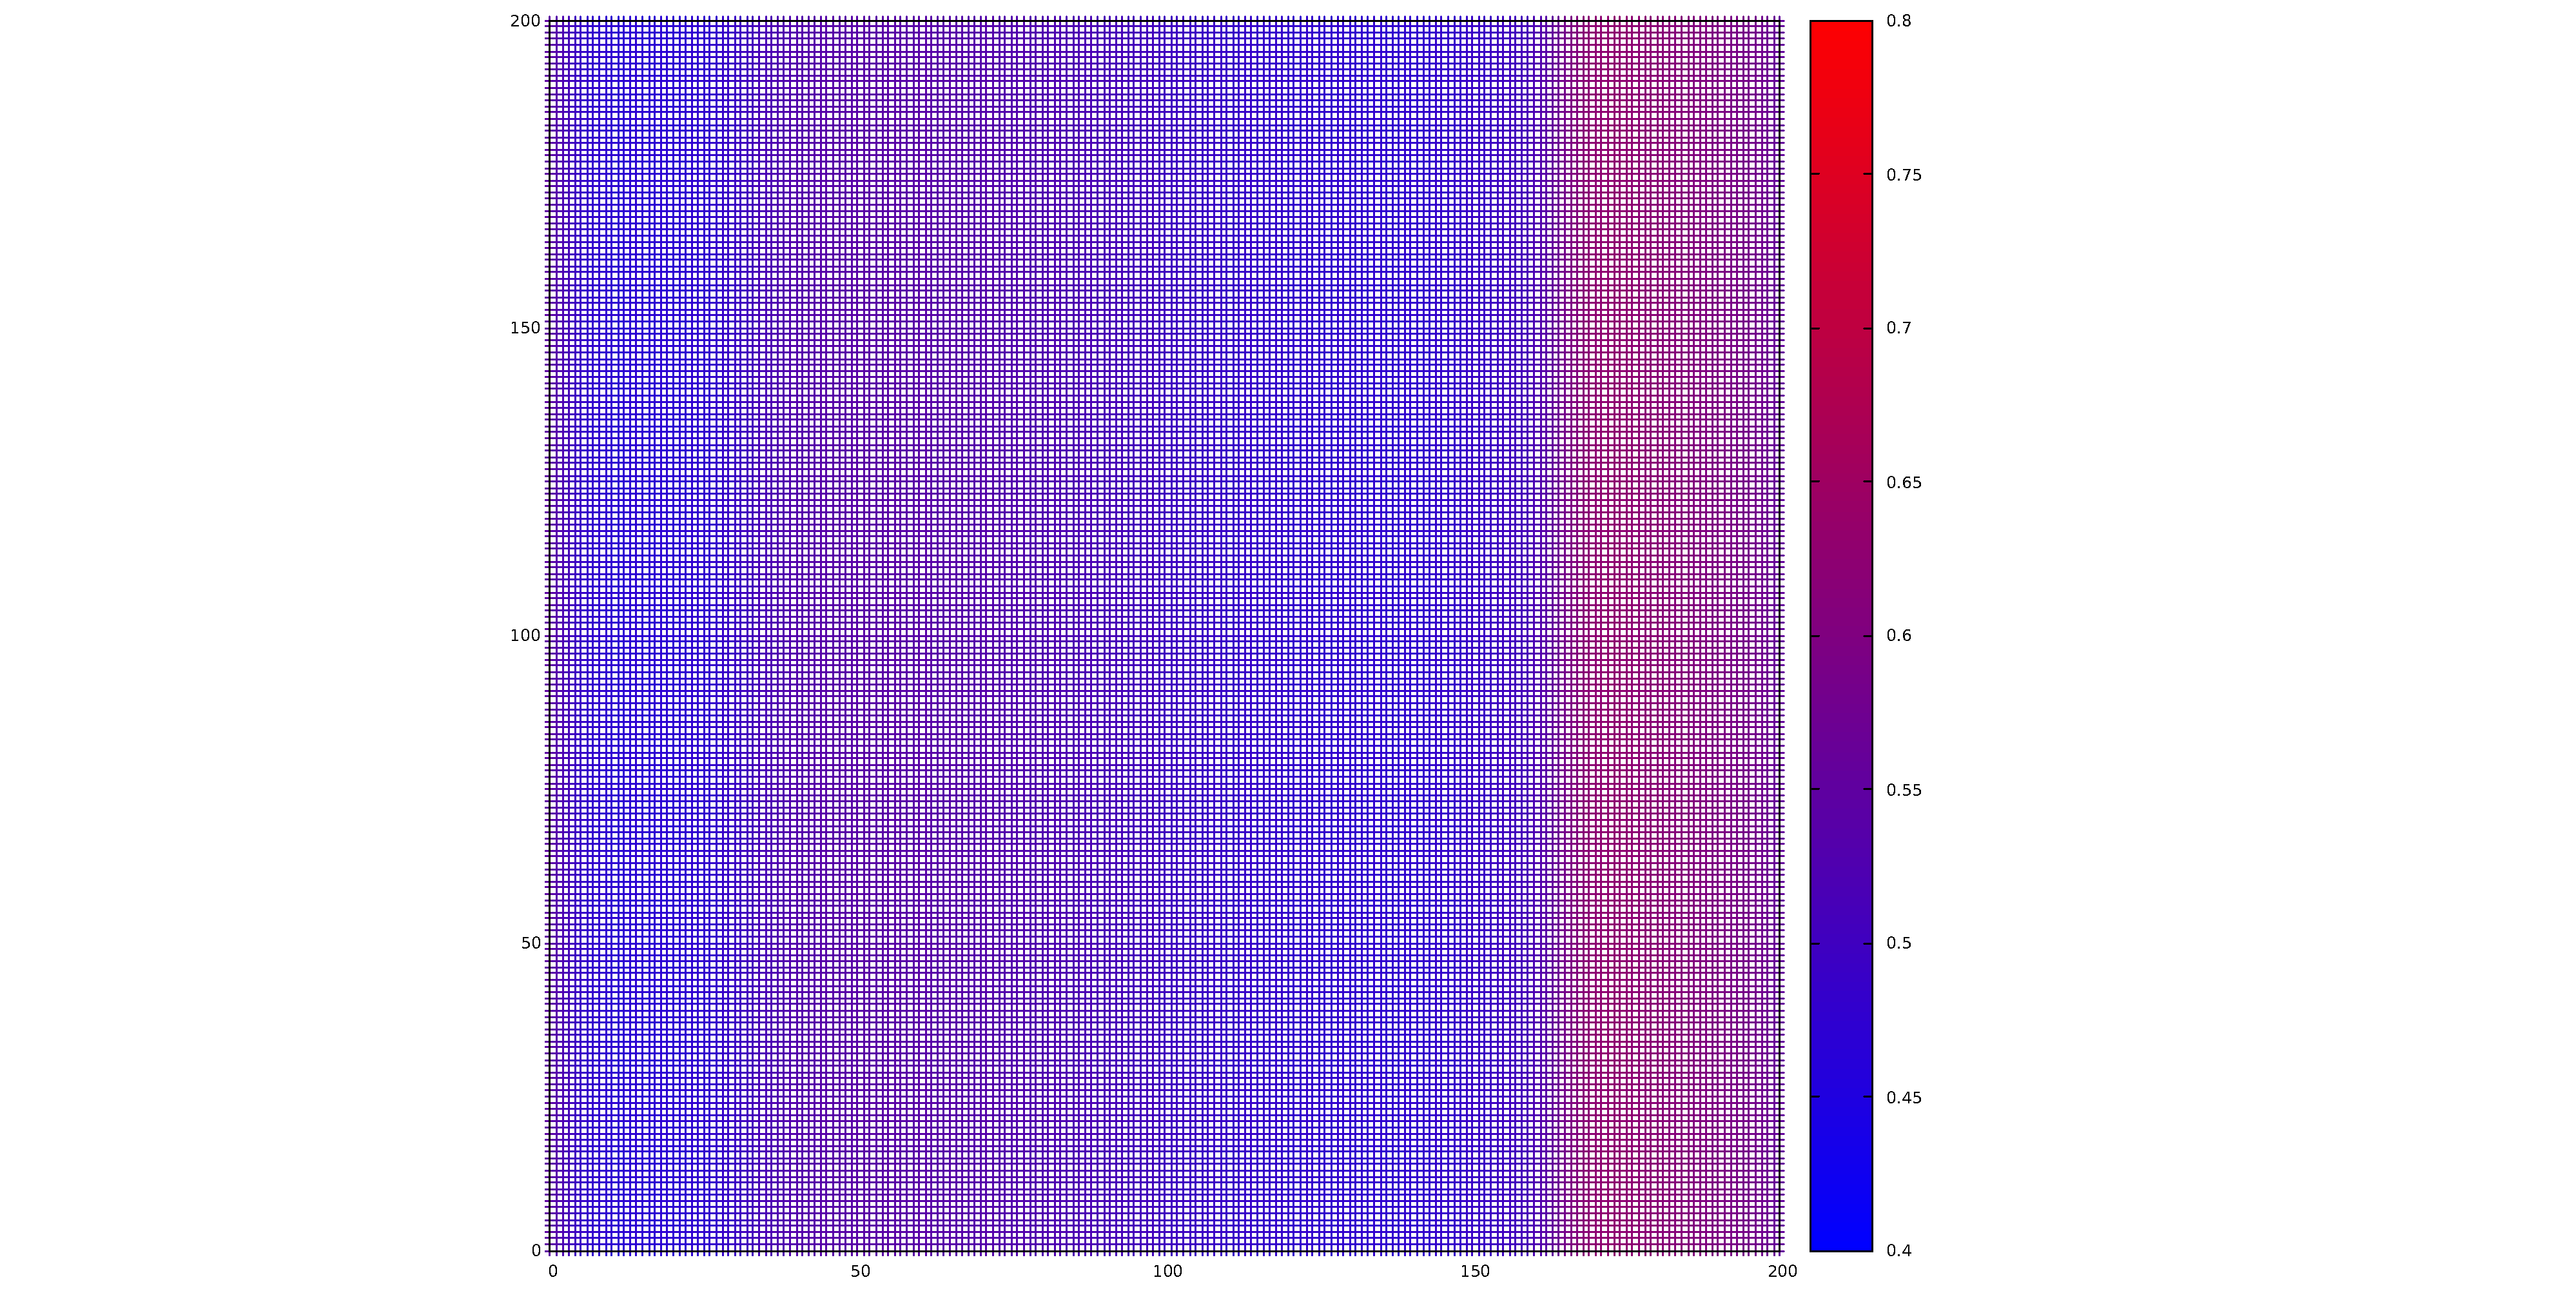
\includegraphics[width=0.4\textwidth]{mapa1000.pdf}
\caption{Mapa bidimensional da densidade. A escala de cores vai de 0.4 (azul) até 0.8 (vermelho). Na primeira linha, da esquerda para a direita, temos os tempos t = 0 e t = 50. Na segunda linha, da esquerda para a direita, temos os tempos t = 200 e t = 1000.}
\label{1b}
\end{figure}

\subsection*{c) }
Apesar de ter gerado os dados sem problemas não consegui encontrar um conjunto de parâmetros adequados para fazer um gráfico satisfatório no gnuplot. As setas sempre ficam pequenas demais. 


\subsection*{d)	}

Na Figura \ref{1d} foi plotado o perfil de densidade $\rho_k$ e o mapa bidimensional para o tempo t = 20000. Os dois gráficos levam à mesma conclusão: $\rho_k$ é aproximadamente constante em todo o espaço, tendo um valor $\rho_k \approx 0.52$.

\begin{figure}[!htb]
\centering
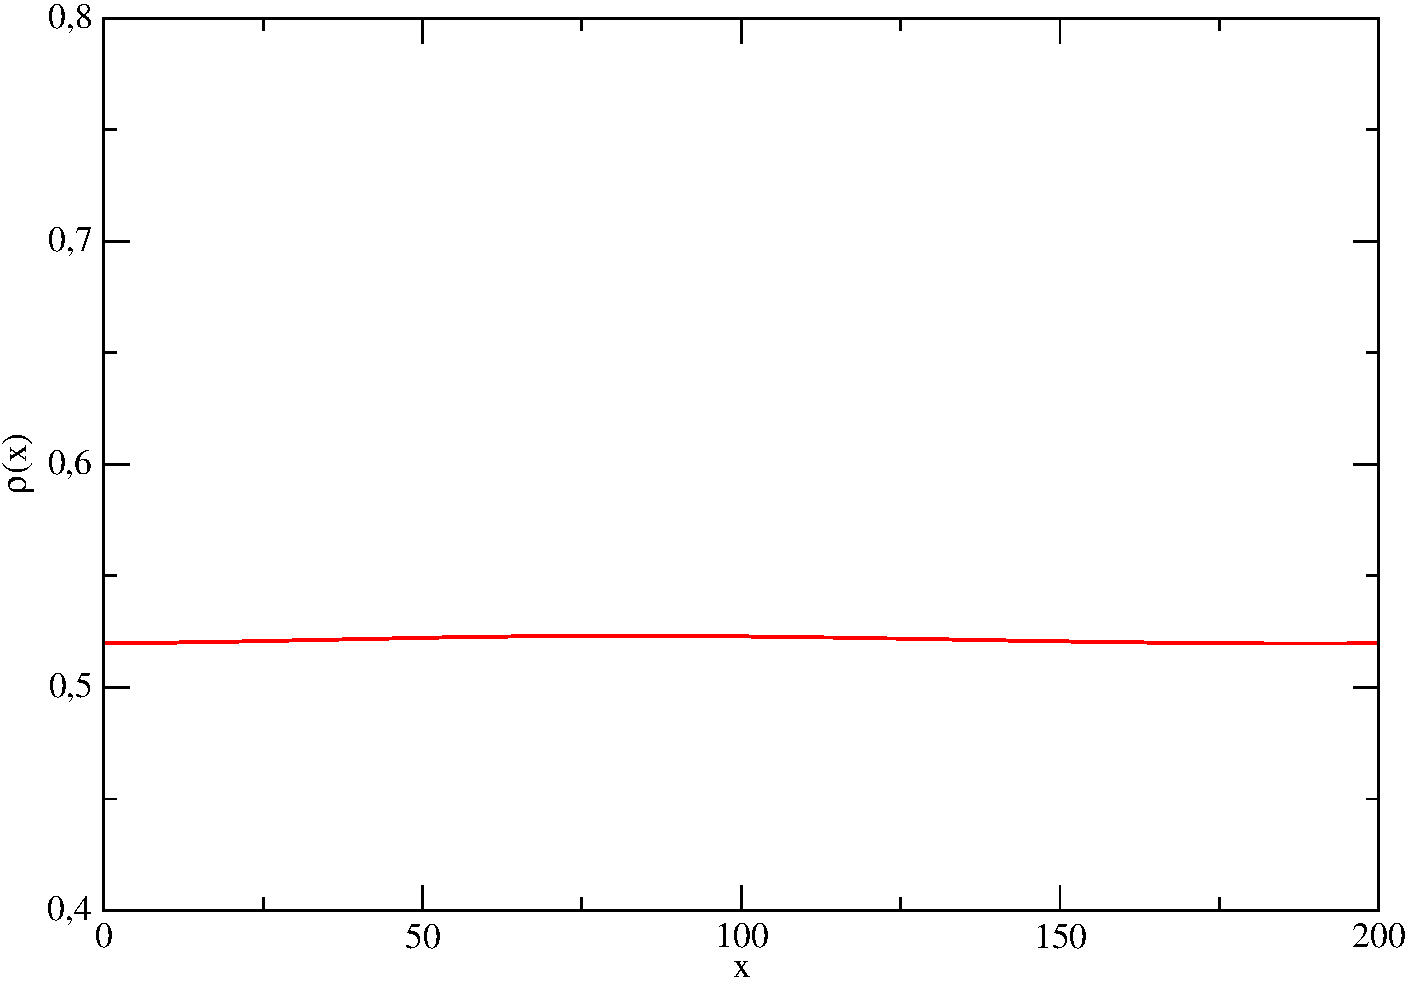
\includegraphics[width=0.35\textwidth]{perfil20000.pdf}
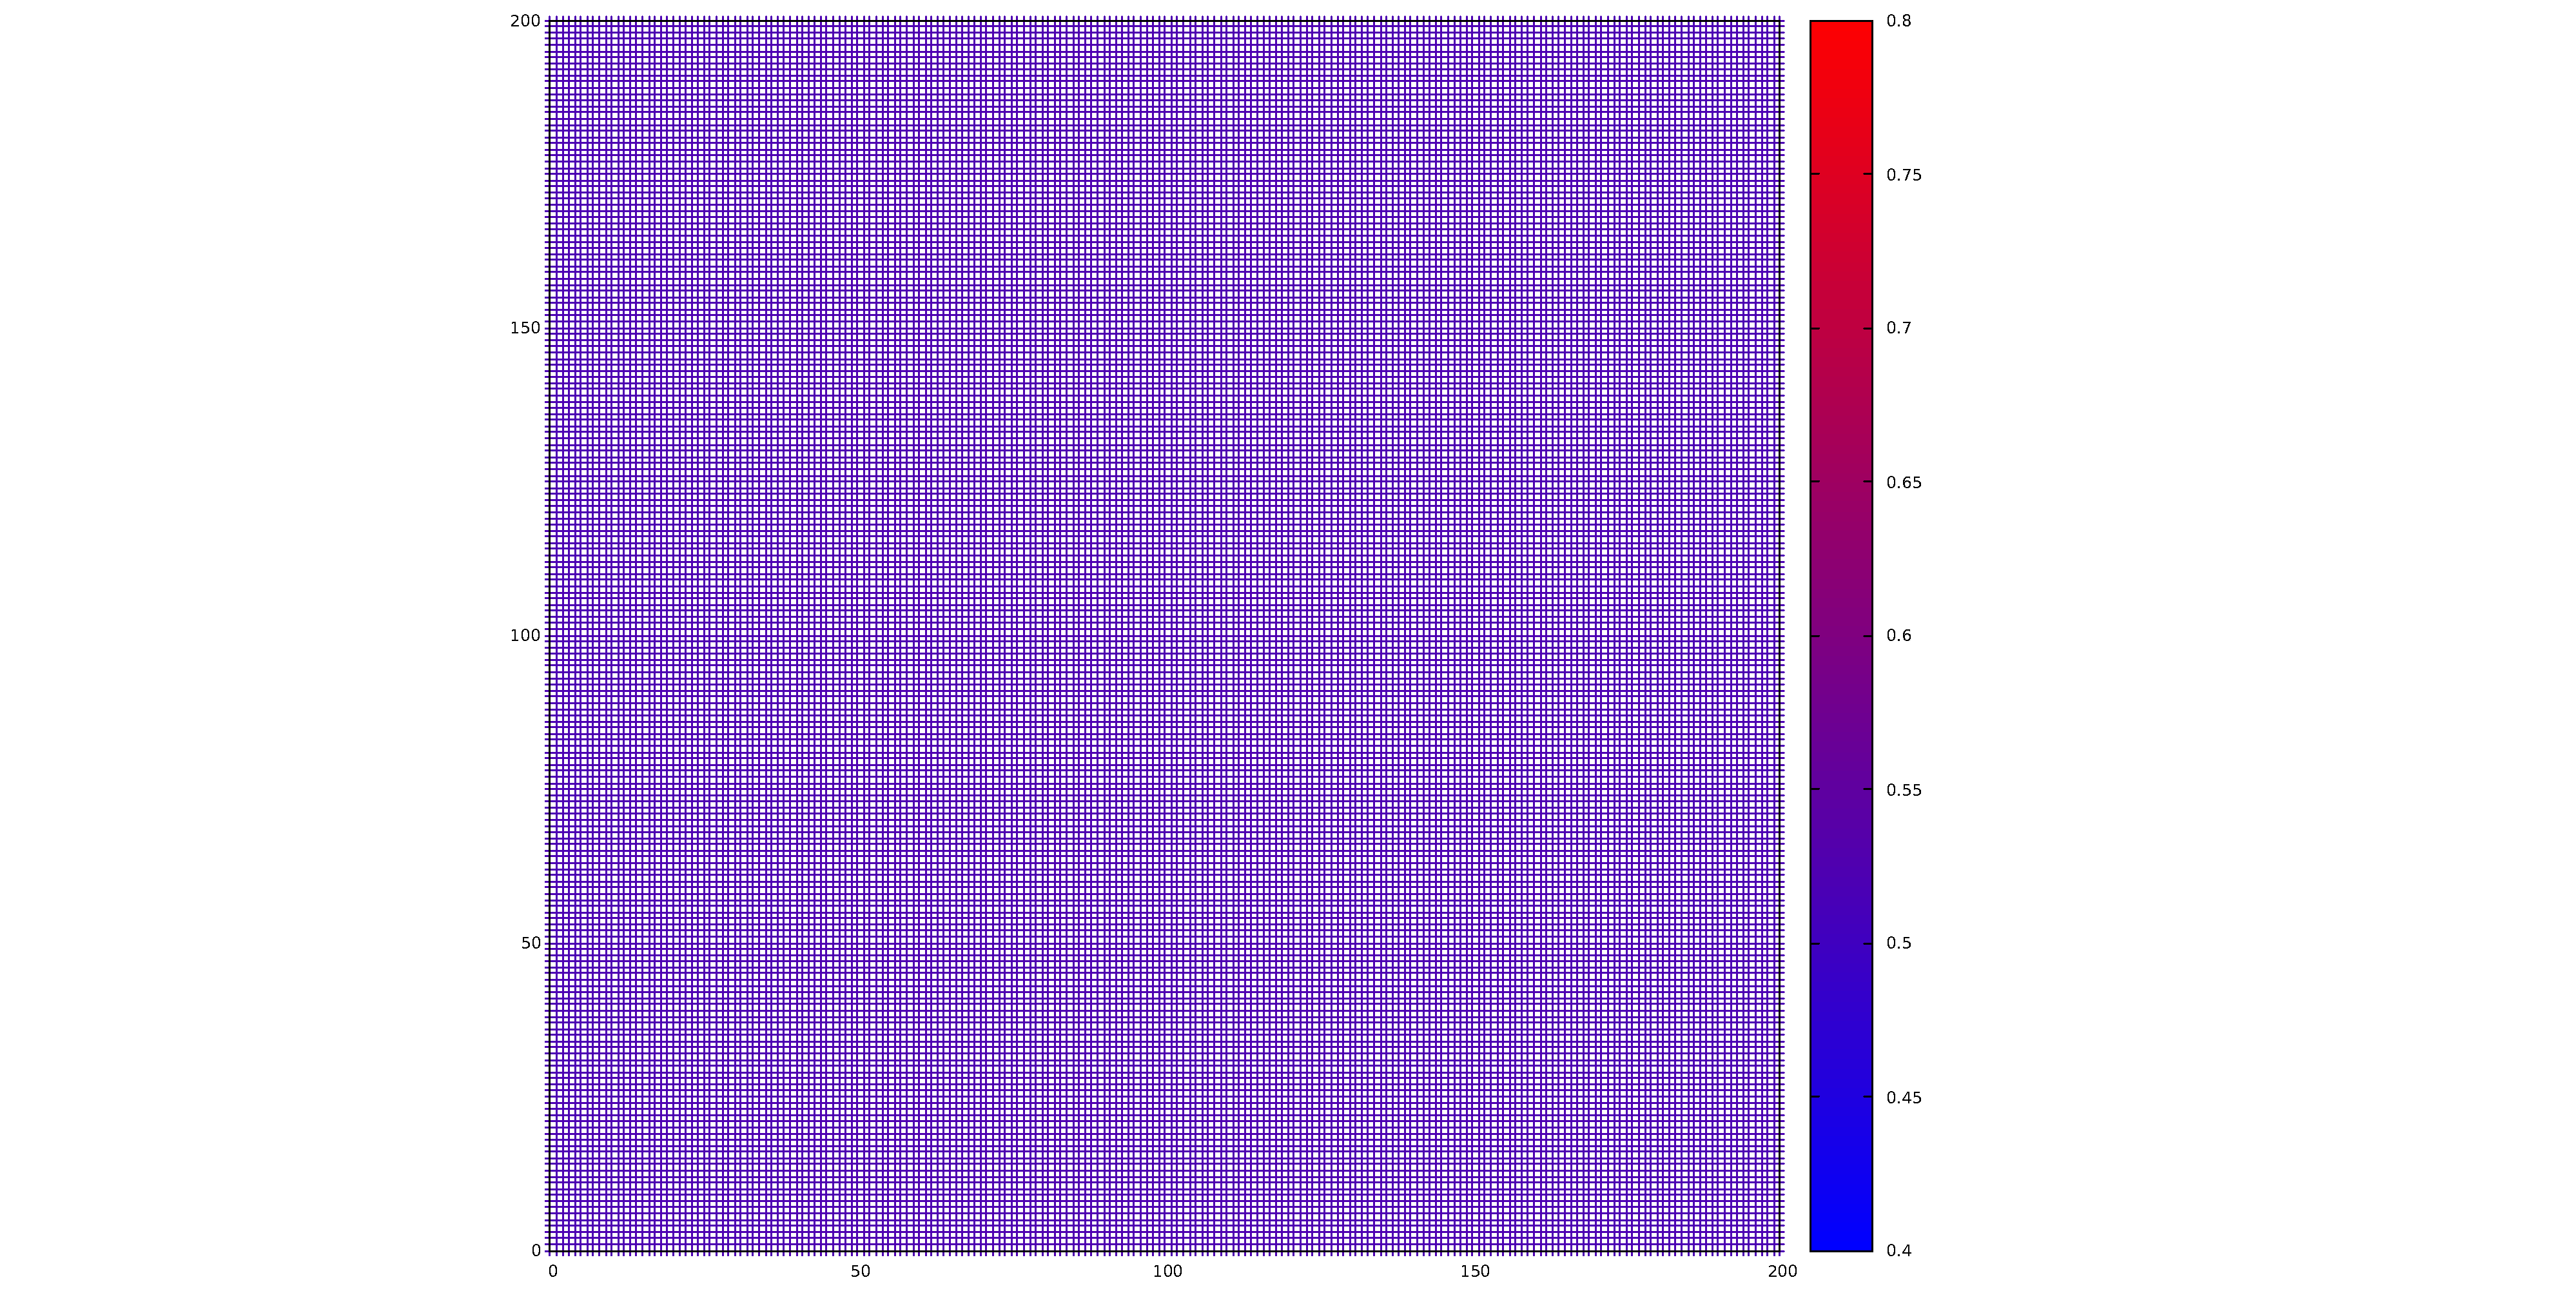
\includegraphics[width=0.5\textwidth]{mapa20000.pdf}
\caption{Perfil de densidade e mapa bidimensional da densidade $\rho_k$ para um tempo t = 20000.}
\label{1d}
\end{figure}


\section*{Exercício 2}
O programa está na pasta 2. Infelizmente houve algum erro na implementação do programa, provavelmente na definição dos vizinhos, e um erro ocorre para tempos $t \approx 40$.

\end{document}